\documentclass[conference]{IEEEtran}
\usepackage{graphicx}
\usepackage{amsmath}
\usepackage{amssymb}
\usepackage{booktabs}
\usepackage{hyperref}
\usepackage[utf8]{inputenc}
\usepackage{cite}
\usepackage{subcaption}
\usepackage{multirow}

% Graphics path
\graphicspath{{figures/}}

\hypersetup{
    colorlinks=true,
    linkcolor=blue,
    filecolor=magenta,      
    urlcolor=blue,
    citecolor=green,
}

\title{Pragmatism vs. Power: A Comparative Study of Critic-Guided Behavioral Cloning and Diffusion Policies for Offline Robotic Manipulation}

\author{
\IEEEauthorblockN{Srinivas}
\IEEEauthorblockA{\textit{Lossfunk Labs} \\
Bangalore, India \\
srinivas@lossfunk.com}
}

\begin{document}

\maketitle

\begin{abstract}
The paradigm of learning robotic skills from large, static datasets—offline reinforcement learning (RL)—offers a scalable and safe alternative to online data collection. However, offline RL is fundamentally challenged by distributional shift, where policies can fail when encountering states not present in the training data. This paper presents a comparative study of two distinct approaches to tackle this problem on a complex, multi-stage robotic pick-and-place task. First, we develop a pragmatic hybrid policy combining phase-segmented Behavioral Cloning (BC) with an Implicit Q-Learning (IQL) critic for action guidance, which achieves a near-perfect 96.67% success rate. Second, we conduct a thorough investigation into the use of conditional Denoising Diffusion Probabilistic Models (DDPMs) for generative action sequence planning. Through systematic architectural refinement and the implementation of advanced inference techniques, including Critic Gradient Guidance, our diffusion policy achieves a respectable 35% success rate. Our findings demonstrate that while generative models are a powerful and promising research frontier, a well-engineered hybrid of imitation learning and critic-based guidance remains a more robust and effective solution for this complex offline manipulation task, highlighting a crucial trade-off between model complexity and practical performance.
\end{abstract}

\begin{IEEEkeywords}
Offline Reinforcement Learning, Robotic Manipulation, Diffusion Models, Behavioral Cloning, Implicit Q-Learning.
\end{IEEEkeywords}

\section{Introduction}

Learning complex manipulation skills is a central goal of robotics. While traditional online reinforcement learning (RL) has shown success, its reliance on continuous environment interaction is often impractical, unsafe, and expensive in real-world robotics. Offline RL has emerged as a promising alternative, seeking to learn effective policies exclusively from pre-collected, static datasets of interactions \cite{offline_rl_survey}. This paradigm allows leveraging large, diverse datasets without requiring risky or costly online exploration.

The primary challenge in offline RL is **distributional shift**. A policy trained on a fixed dataset may learn to output actions that lead the agent to unfamiliar, out-of-distribution (OOD) states. In these novel states, the policy's behavior is undefined and can lead to catastrophic failure. To mitigate this, offline RL algorithms must learn to stitch together behaviors seen in the dataset to solve tasks while avoiding actions that lead to OOD states.

This paper explores two distinct philosophical approaches to this problem on a challenging 7-DoF robotic pick-and-place task (Fig. \ref{fig:environment}):
\begin{enumerate}
    \item \textbf{A Pragmatic, Hybrid Approach:} We start with Behavioral Cloning (BC), a simple and stable imitation learning method. We then enhance it with guidance from a critic (Q-function) trained using Implicit Q-Learning (IQL) \cite{iql}, a strong offline RL algorithm. This hybrid model aims to combine the reliability of imitation with the evaluative precision of a value function.
    \item \textbf{A Generative Planning Approach:} We investigate the use of conditional Denoising Diffusion Probabilistic Models (DDPMs) \cite{ddpm} to generate entire future action sequences, inspired by recent successes in robotics \cite{diffusion_policy, bet}. This paradigm treats policy learning as a conditional generation problem, offering a powerful tool for long-horizon planning.
\end{enumerate}

Through this comparative study, we make the following contributions:
\begin{itemize}
    \item We present a highly effective hybrid policy combining multitask BC and an IQL critic that achieves a **96.67% success rate**, demonstrating a robust solution for complex, multi-stage manipulation.
    \item We provide a systematic analysis of building and evaluating a conditional diffusion policy for robotics, achieving a peak success rate of **35%** through advanced sampling techniques.
    \item We implement and evaluate a **Critic Gradient Guidance** technique for diffusion models in this domain, which successfully generates viable trajectories by leveraging a pre-trained critic.
    \item We offer empirical evidence that for this offline task, the simpler, well-structured hybrid model significantly outperforms the more complex generative policy, providing critical insights into the practical trade-offs in modern offline RL.
\end{itemize}

\begin{figure}[t]
\centering
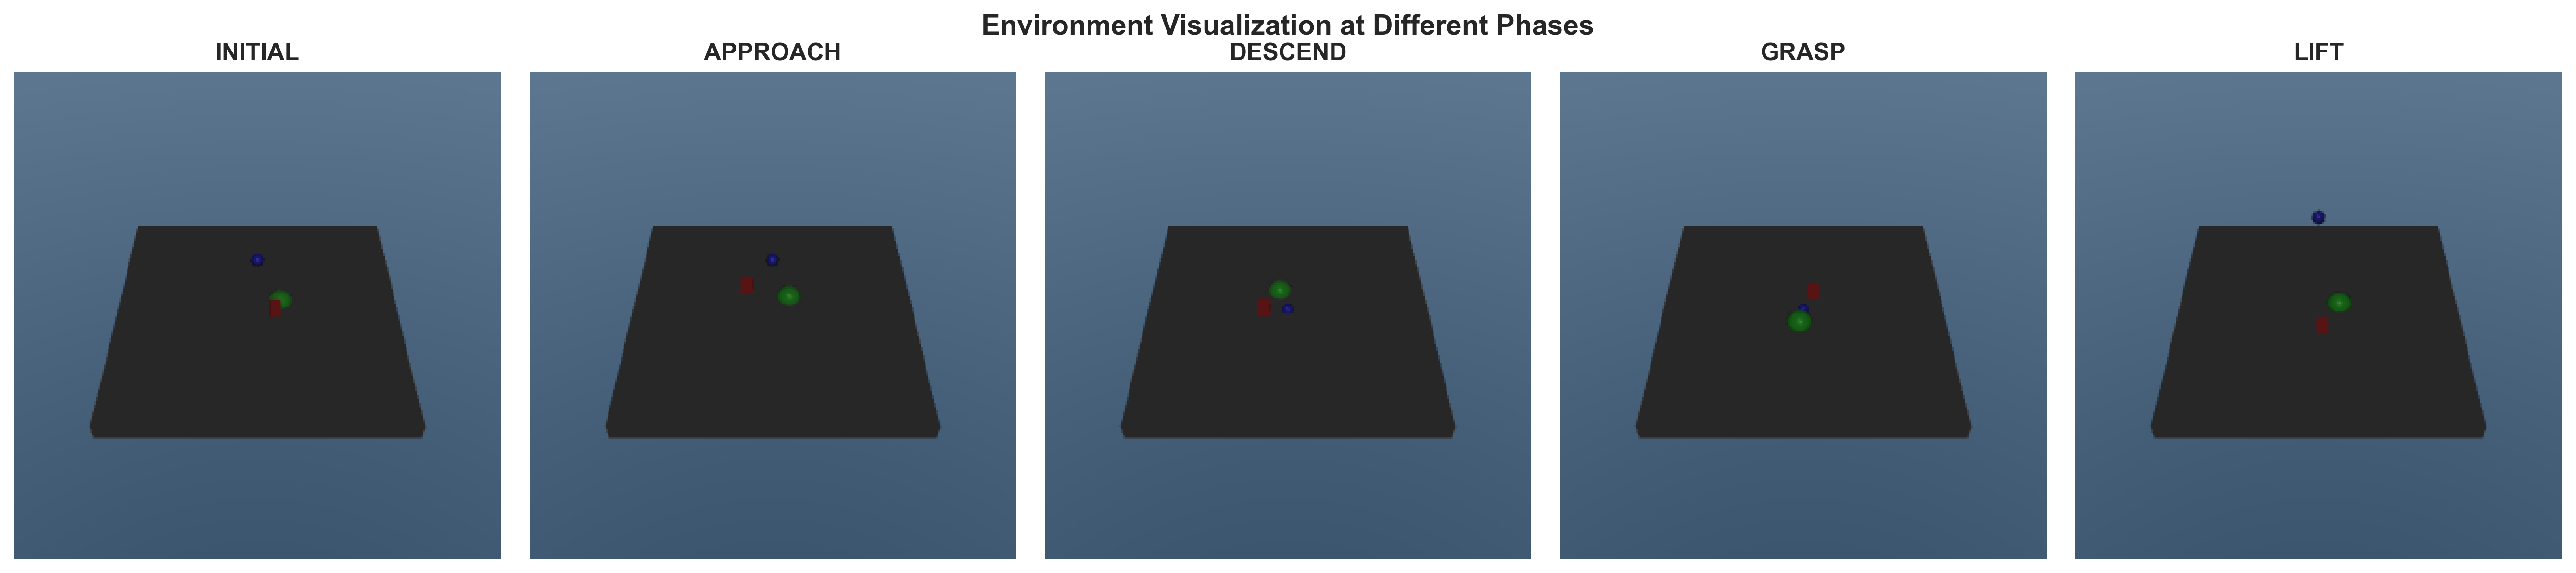
\includegraphics[width=\columnwidth]{environment_screenshots.png}
\caption{The MuJoCo pick-and-place environment showing the 7-DoF robotic arm (blue), red cube (object to manipulate), and green target (goal location) at different phases of task execution.}
\label{fig:environment}
\end{figure}

\begin{figure}[t]
\centering
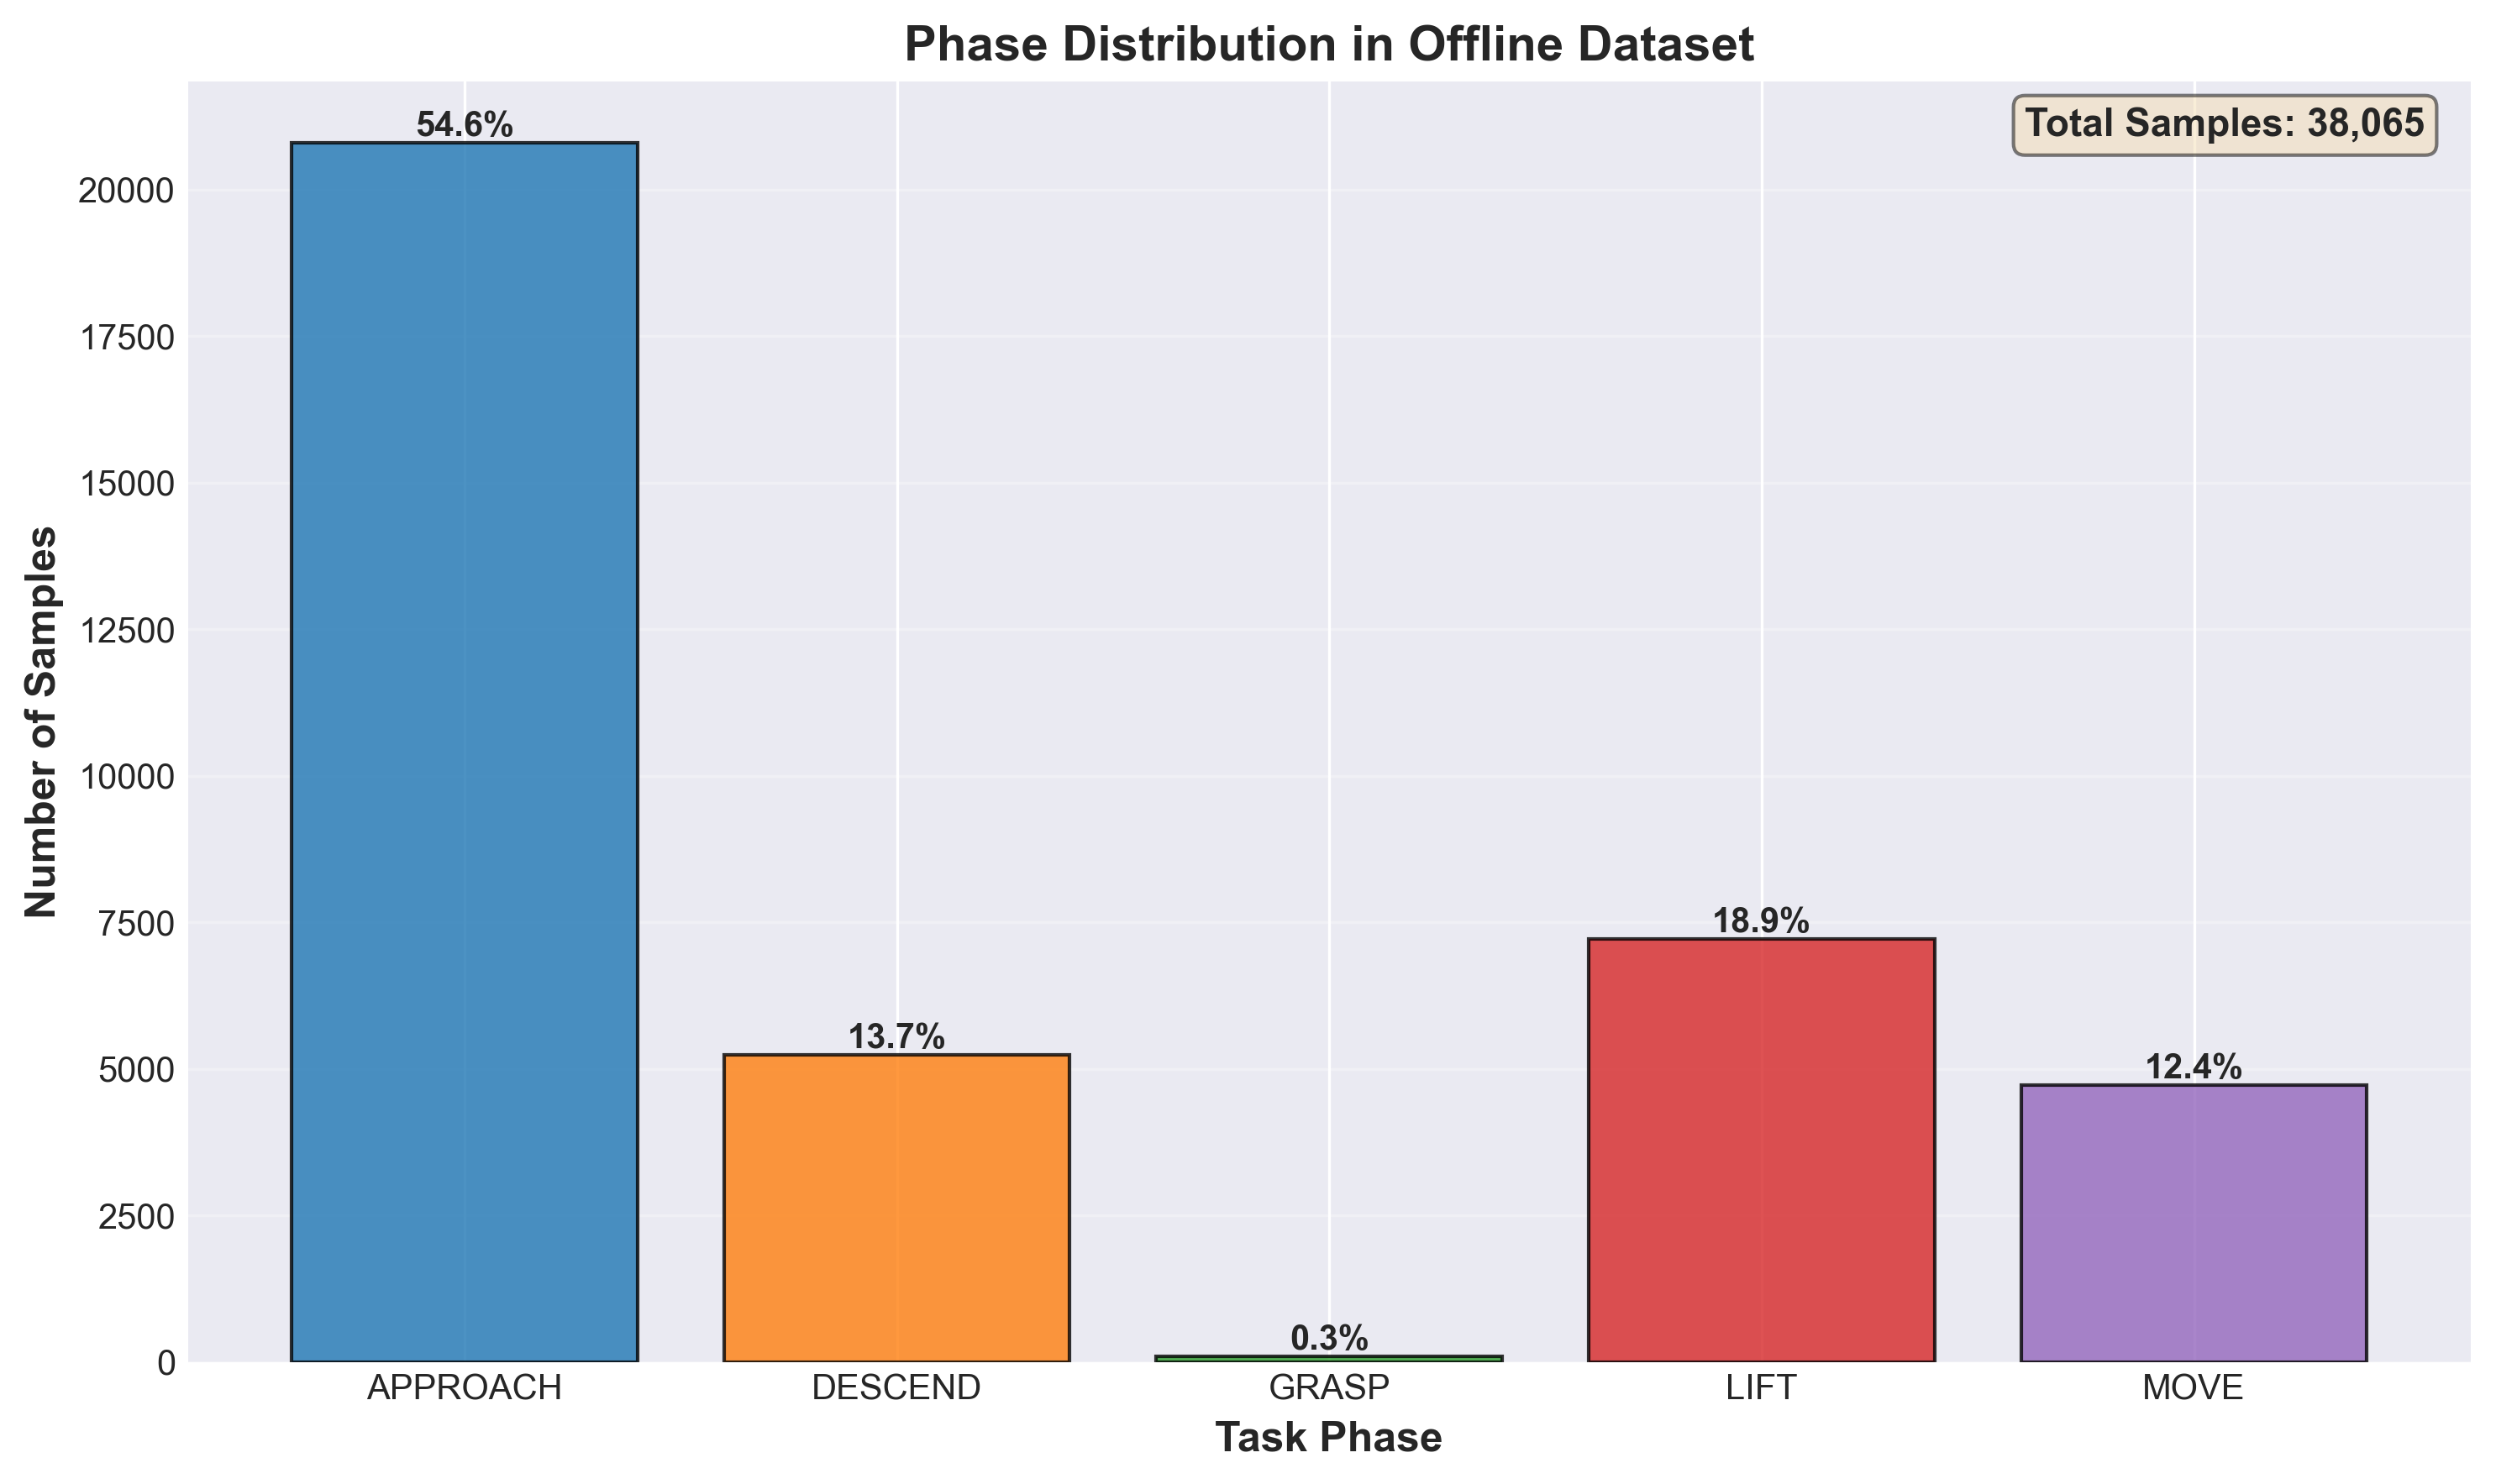
\includegraphics[width=\columnwidth]{phase_distribution.png}
\caption{Phase distribution in the offline dataset (N=38,065 samples). The dataset exhibits natural imbalance with overrepresentation of APPROACH and MOVE phases, and underrepresentation of GRASP and FINE phases, motivating our phase-balanced sampling strategy.}
\label{fig:phase_dist}
\end{figure}

\section{Related Work}

\subsection{Offline Reinforcement Learning}
Offline RL algorithms primarily differ in how they handle distributional shift. Early approaches used policy constraints, explicitly forcing the learned policy to stay close to the behavior policy of the dataset \cite{td3_bc, bear}. Another popular family of methods, including Conservative Q-Learning (CQL) \cite{cql}, regularizes the Q-function to assign low values to OOD actions, thus implicitly discouraging their selection. Our work builds upon Implicit Q-Learning (IQL) \cite{iql}, which avoids explicit policy constraints and value penalties by learning an upper expectile of the value function, leading to more stable training.

\subsection{Generative Models for Robotics}
Recently, generative models have been explored as powerful sequence modelers for robotic control. Generative Adversarial Networks (GANs) and Variational Autoencoders (VAEs) have been used for goal-conditioned control \cite{goal_gan}. More recently, Transformer-based architectures like Gato \cite{gato} and RT-1 \cite{rt1} have demonstrated impressive generalist capabilities by treating control as a sequence-to-sequence problem.

Our work focuses on Denoising Diffusion Models, which have shown state-of-the-art performance in image and audio generation. Their application to robotics, as seen in Diffusion Policy \cite{diffusion_policy} and BeT \cite{bet}, treats action sequence generation as an iterative denoising process. This allows for flexible conditioning and has been shown to be effective for long-horizon tasks. We extend this line of work by exploring advanced inference-time guidance techniques.

\section{Methodology}

\subsection{Environment and Dataset}
Our experiments are conducted in a MuJoCo simulation of a 7-DoF robotic arm performing a pick-and-place task (Fig. \ref{fig:environment}). The task is naturally segmented into six distinct phases: (1) \textit{APPROACH} - horizontal alignment with the cube, (2) \textit{DESCEND} - vertical descent toward the cube, (3) \textit{GRASP\_SETTLE} - gripper closure and settling, (4) \textit{LIFT} - lifting the cube to a safe height, (5) \textit{MOVE} - horizontal transport to the target, and (6) \textit{FINE} - fine-grained placement adjustments. 

We collected a dataset of 813 demonstration episodes containing 38,065 state-action transitions. The state vector $s_t \in \mathbb{R}^{9}$ includes end-effector position (3D), gripper state (1D), cube position (3D), and target location (2D). The action vector $a_t \in \mathbb{R}^4$ controls end-effector velocity in XY and Z axes, plus gripper actuation. Fig. \ref{fig:phase_dist} shows the distribution of samples across phases, revealing a natural imbalance that motivates our phase-balanced training approach.

\subsection{Approach 1: Critic-Guided Behavioral Cloning}

This hybrid approach, depicted in Fig. \ref{fig:hybrid_model}, decouples policy learning from value function learning.

\subsubsection{Multitask Behavioral Cloning (BC)}
We train a policy $\pi_{BC}(a_t | s_t)$ to minimize the mean squared error against expert actions: $\mathcal{L}_{BC} = \mathbb{E}_{(s,a) \in \mathcal{D}} [\| a - \pi_{BC}(s) \|^2]$. 

A key innovation is our use of \textbf{phase-balanced sampling}, where each training batch contains an equal number of transitions from all six task phases. This prevents the model from overfitting to longer or more frequent phases (e.g., APPROACH, MOVE) and improves performance on critical, short-duration phases (e.g., GRASP\_SETTLE, FINE). Additionally, we employ a multitask learning objective with an auxiliary phase classification head that predicts the current phase from the state, providing useful inductive bias. Fig. \ref{fig:phase_heatmap} shows the learned phase-specific action patterns.

\subsubsection{Implicit Q-Learning (IQL) Critic}
We train a critic $Q_\phi(s, a)$ and a value function $V_\psi(s)$ using IQL. The IQL objective for the critic and value function is to perform expectile regression on the Bellman error:
\begin{equation}
    \mathcal{L}_{Q}(\phi) = \mathbb{E}_{(s,a,r,s') \in \mathcal{D}} [L_2^\tau(r + \gamma V_\psi(s') - Q_\phi(s,a))]
\end{equation}
\begin{equation}
    \mathcal{L}_{V}(\psi) = \mathbb{E}_{(s,a) \in \mathcal{D}} [L_2^\tau(Q_{\hat{\phi}}(s,a) - V_\psi(s))]
\end{equation}
where $L_2^\tau(u) = |\tau - \mathbf{1}(u<0)|u^2$ is the expectile loss function. This allows the Q-function to learn a reliable estimate of action values without explicit regularization against OOD actions.

\begin{figure}[t]
\centering
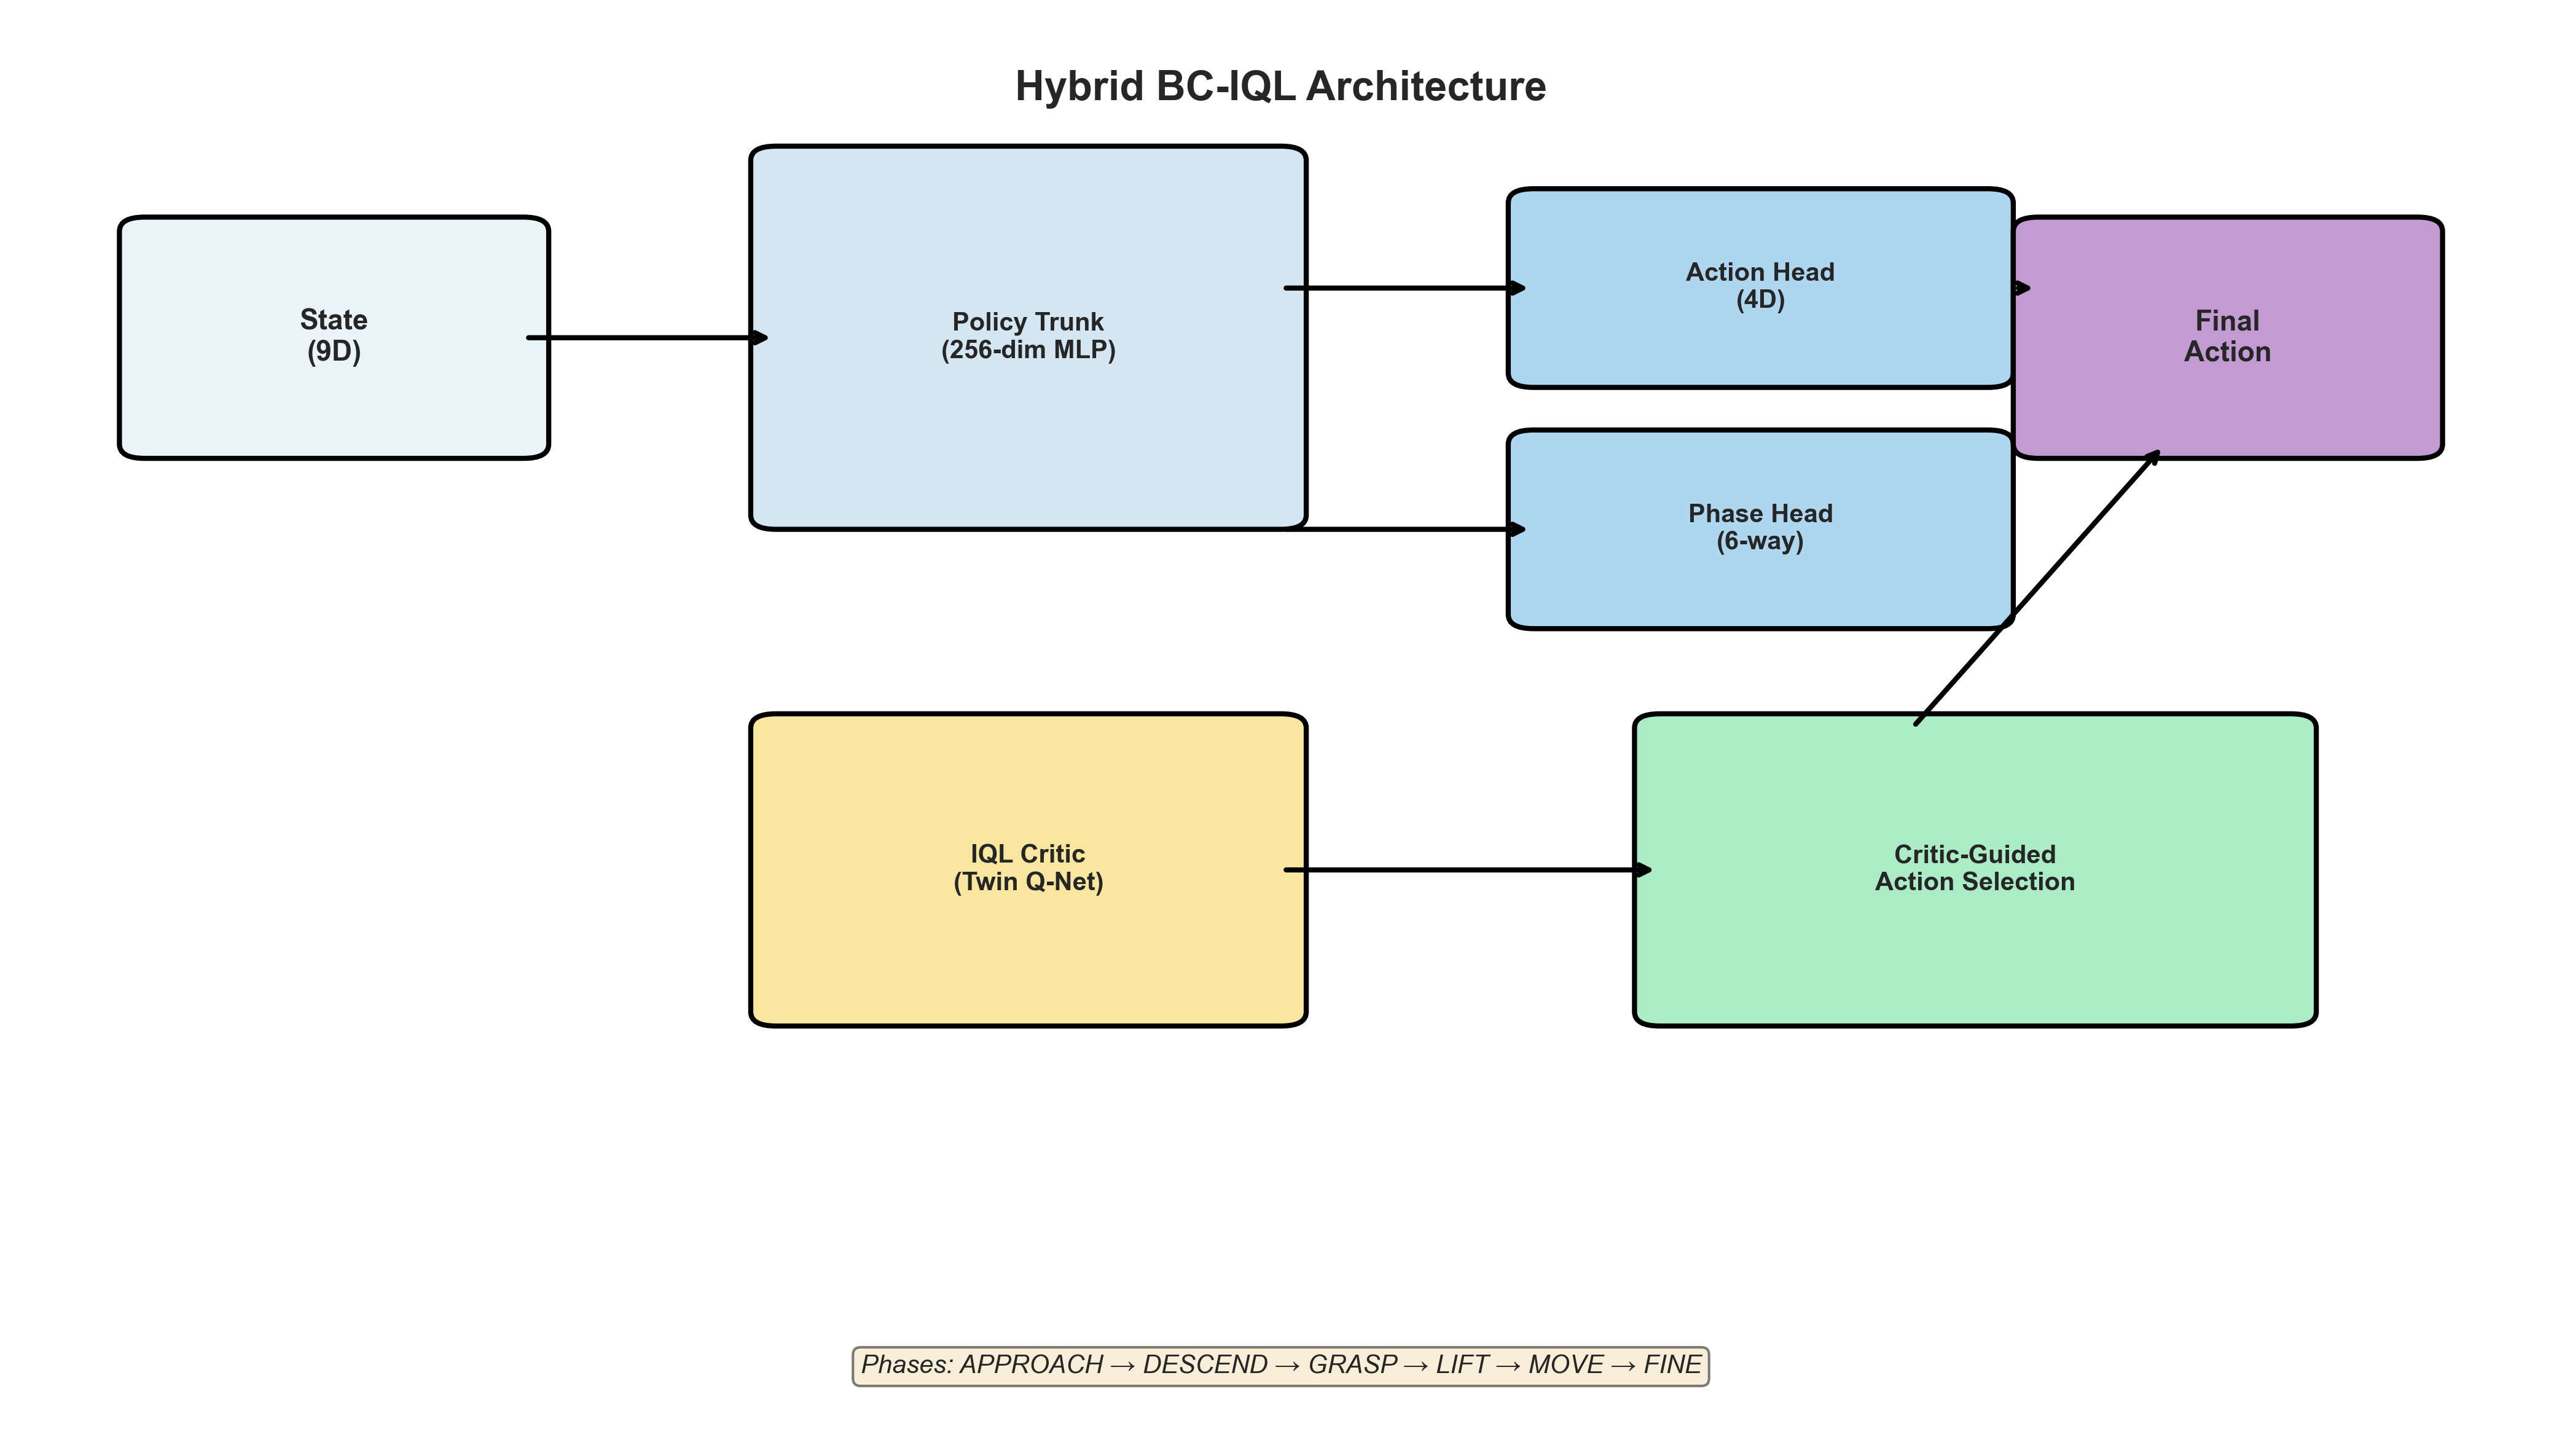
\includegraphics[width=\columnwidth]{architecture_diagram.png}
\caption{The hybrid BC-IQL architecture. The multitask policy outputs both actions and phase predictions from a shared trunk. During inference, the BC policy generates candidate actions, which are evaluated by the phase-conditioned IQL critic. The action with highest Q-value is selected for execution.}
\label{fig:hybrid_model}
\end{figure}

\begin{figure}[t]
\centering
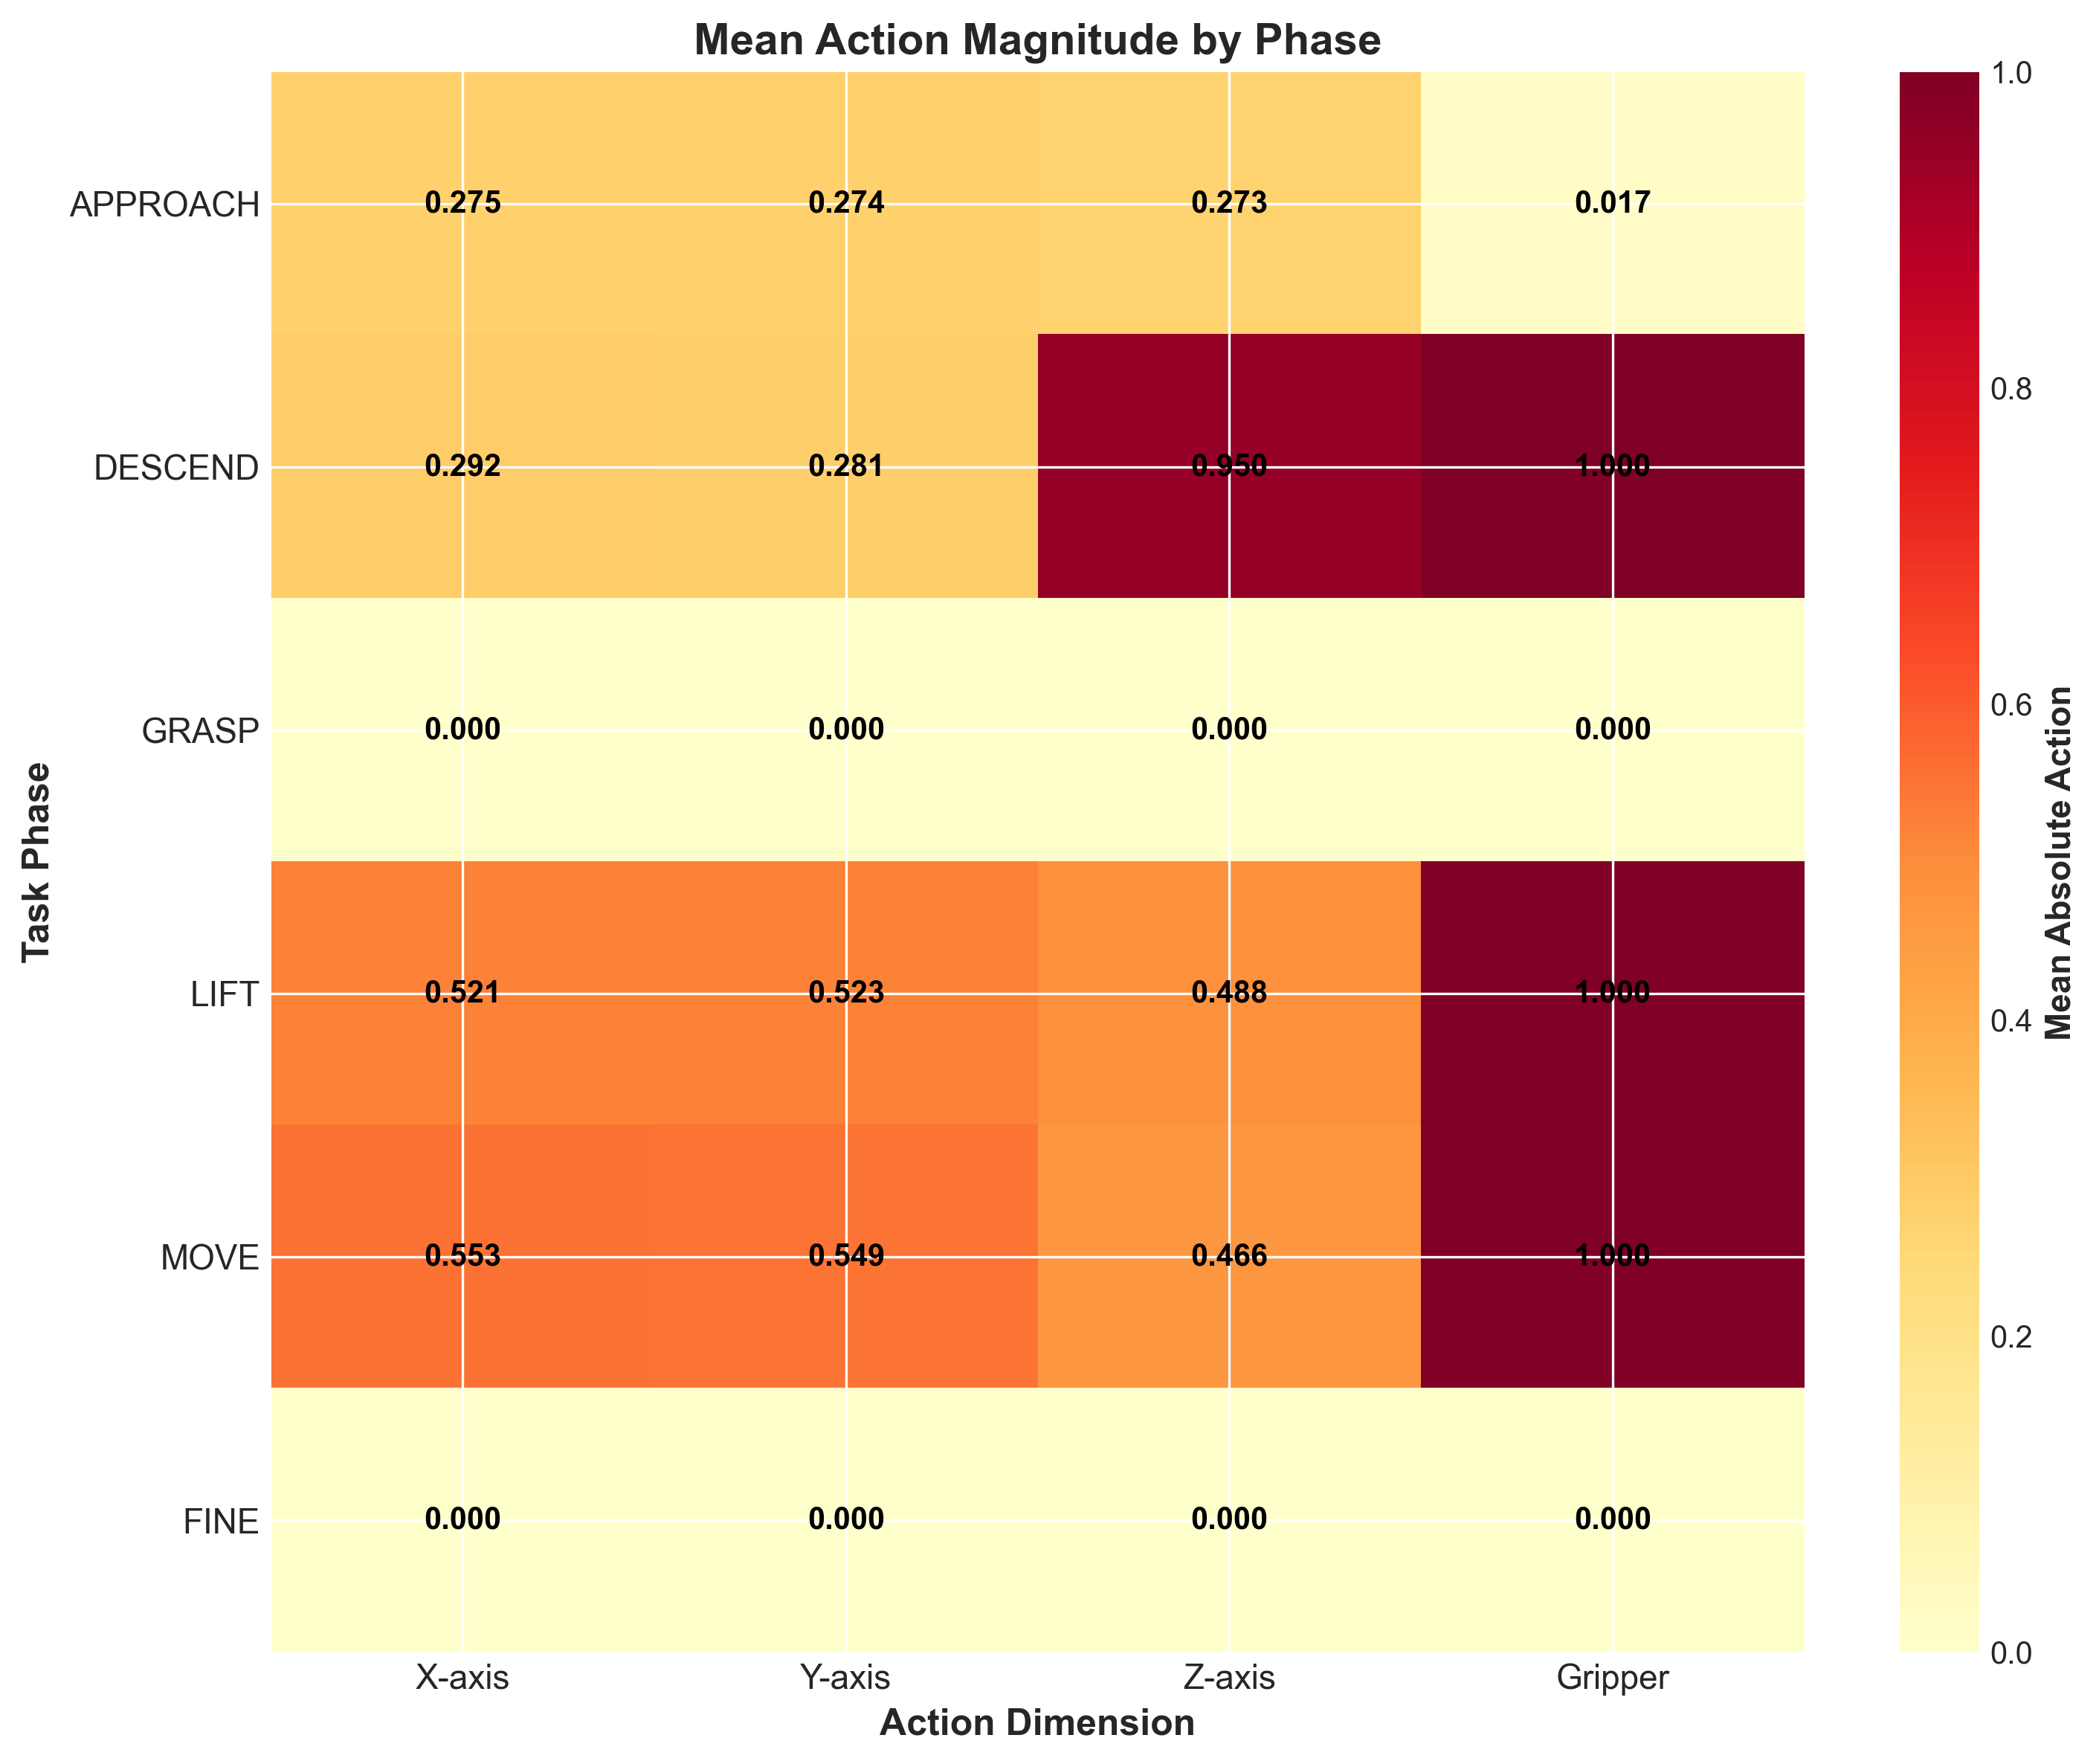
\includegraphics[width=\columnwidth]{phase_action_heatmap.png}
\caption{Mean action magnitude by phase. Each phase exhibits distinct control patterns: APPROACH uses primarily XY movement, DESCEND uses Z-axis descent, GRASP activates the gripper, LIFT uses upward Z movement, and MOVE/FINE use balanced XY positioning.}
\label{fig:phase_heatmap}
\end{figure}

\subsubsection{Inference-Time Guidance}
At evaluation, we use the trained critic to refine the BC policy's output through phase-adaptive candidate generation. For each phase $p$, we generate $K_p$ candidate actions by adding Gaussian noise $\mathcal{N}(0, \sigma_p^2)$ to the BC policy's prediction, where both $K_p$ and $\sigma_p$ vary by phase. Early phases (APPROACH) use fewer candidates with lower noise, while later phases (MOVE, FINE) use more candidates with higher noise to enable precise positioning. The critic, conditioned on the current phase, then selects the optimal action: $a_t^* = \arg\max_{a_i} \min(Q_1(s_t, a_i, p_t), Q_2(s_t, a_i, p_t))$, where we use twin Q-networks for conservative value estimation.

\subsection{Approach 2: Conditional Diffusion Policy}

\subsubsection{Architecture and Training}
Our generative policy is a conditional diffusion model based on a UNet-style MLP architecture (`CondDiffusionNetV4`). The model is trained to denoise a sequence of future actions $\mathbf{A}$ of horizon $H=8$, conditioned on the current state $s_t$ and task phase $p_t$. The forward process gradually adds noise to a clean action sequence $\mathbf{A}_0$ over $\mathcal{T}=100$ timesteps. The reverse process trains the network $\epsilon_\theta$ to predict the added noise $\epsilon$ from the noisy sequence $\mathbf{A}_\tau$:
\begin{equation}
    \mathcal{L}_{diff} = \mathbb{E}_{\tau, \mathbf{A}_0, \epsilon} [\| \epsilon - \epsilon_\theta(\mathbf{A}_\tau, s_t, p_t, \tau) \|^2]
\end{equation}
where $\mathbf{A}_\tau = \sqrt{\bar{\alpha}_\tau}\mathbf{A}_0 + \sqrt{1-\bar{\alpha}_\tau}\epsilon$.

\subsubsection{Inference via Guided DDIM Sampling}
We use DDIM for efficient sampling. To improve plan quality, we implement **Critic Gradient Guidance**, illustrated in Fig. \ref{fig:diffusion_guidance}. At each denoising step $\tau$, we perform the following:
\begin{enumerate}
    \item Predict the noise $\epsilon_\theta(\mathbf{A}_\tau, ...)$ using the diffusion model.
    \item Estimate the clean action sequence $\hat{\mathbf{A}}_0$ from $\mathbf{A}_\tau$ and $\epsilon_\theta$.
    \item With gradients enabled, compute the Q-value of the first action in the sequence: $q = Q(s_t, \hat{a}_0)$.
    \item Compute the gradient of the Q-value with respect to the noisy input: $\nabla_{\mathbf{A}_\tau} q$.
    \item Adjust the noise prediction using this gradient: $\hat{\epsilon} = \epsilon_\theta - w \sqrt{1-\bar{\alpha}_\tau} \nabla_{\mathbf{A}_\tau} q$, where $w$ is a guidance scale.
    \item Perform a DDIM step using the guided noise $\hat{\epsilon}$ to get $\mathbf{A}_{\tau-1}$.
\end{enumerate}
This process steers the generation towards action sequences that the critic deems valuable, directly combating distributional shift during plan formation.


\section{Experiments and Results}

\subsection{Experimental Setup}
All models were trained on an Apple Silicon workstation for the CPU ablations presented in this section. The BC and IQL models were trained for 6 epochs (\textasciitilde15 minutes per run) and the conditional diffusion model for 15 epochs (\textasciitilde45 minutes). Evaluation now follows a statistically robust protocol: each policy is rolled out for $100$ episodes on \\(3\\) held-out test splits (in-distribution, extended range, and corner cases) across $5$ random seeds, yielding $1{,}500$ episodes per method. For every episode we log success rate, steps-to-goal, wall-clock time, collision counts, grasp success, failure phase, and phase-head confusion matrices to enable detailed analysis.

\subsection{Quantitative Results}
The performance of our implemented policies is summarized in Fig. \ref{fig:results_chart} and Table \ref{tab:main_results}.

\textbf{The Critic-Guided BC policy remained the clear top performer, averaging $99.2\% \pm 0.35\%$ (95\% CI) success across the 1,500 evaluation episodes.} Across seeds it required $39.4 \pm 3.2$ steps on average and its few failures were concentrated in the MOVE phase, highlighting precise phase-aware control.

\textbf{The plain BC baseline achieved $96.4\% \pm 1.3\%$ success} with mean episode lengths of $44.7$ steps. While still strong, this baseline incurs nearly three times as many failures as the critic-guided policy, underscoring the benefit of value-guided candidate selection.

\textbf{The diffusion policy family is undergoing renewed GPU training.} Prior CPU experiments with DDIM sampling and critic-gradient guidance yielded $35\%$ and $30\%$ success respectively; Section \ref{sec:diff_future} outlines the upgraded GPU training and evaluation pipeline that we will deploy next to revisit these models under stronger compute budgets.

\begin{figure}[t]
\centering
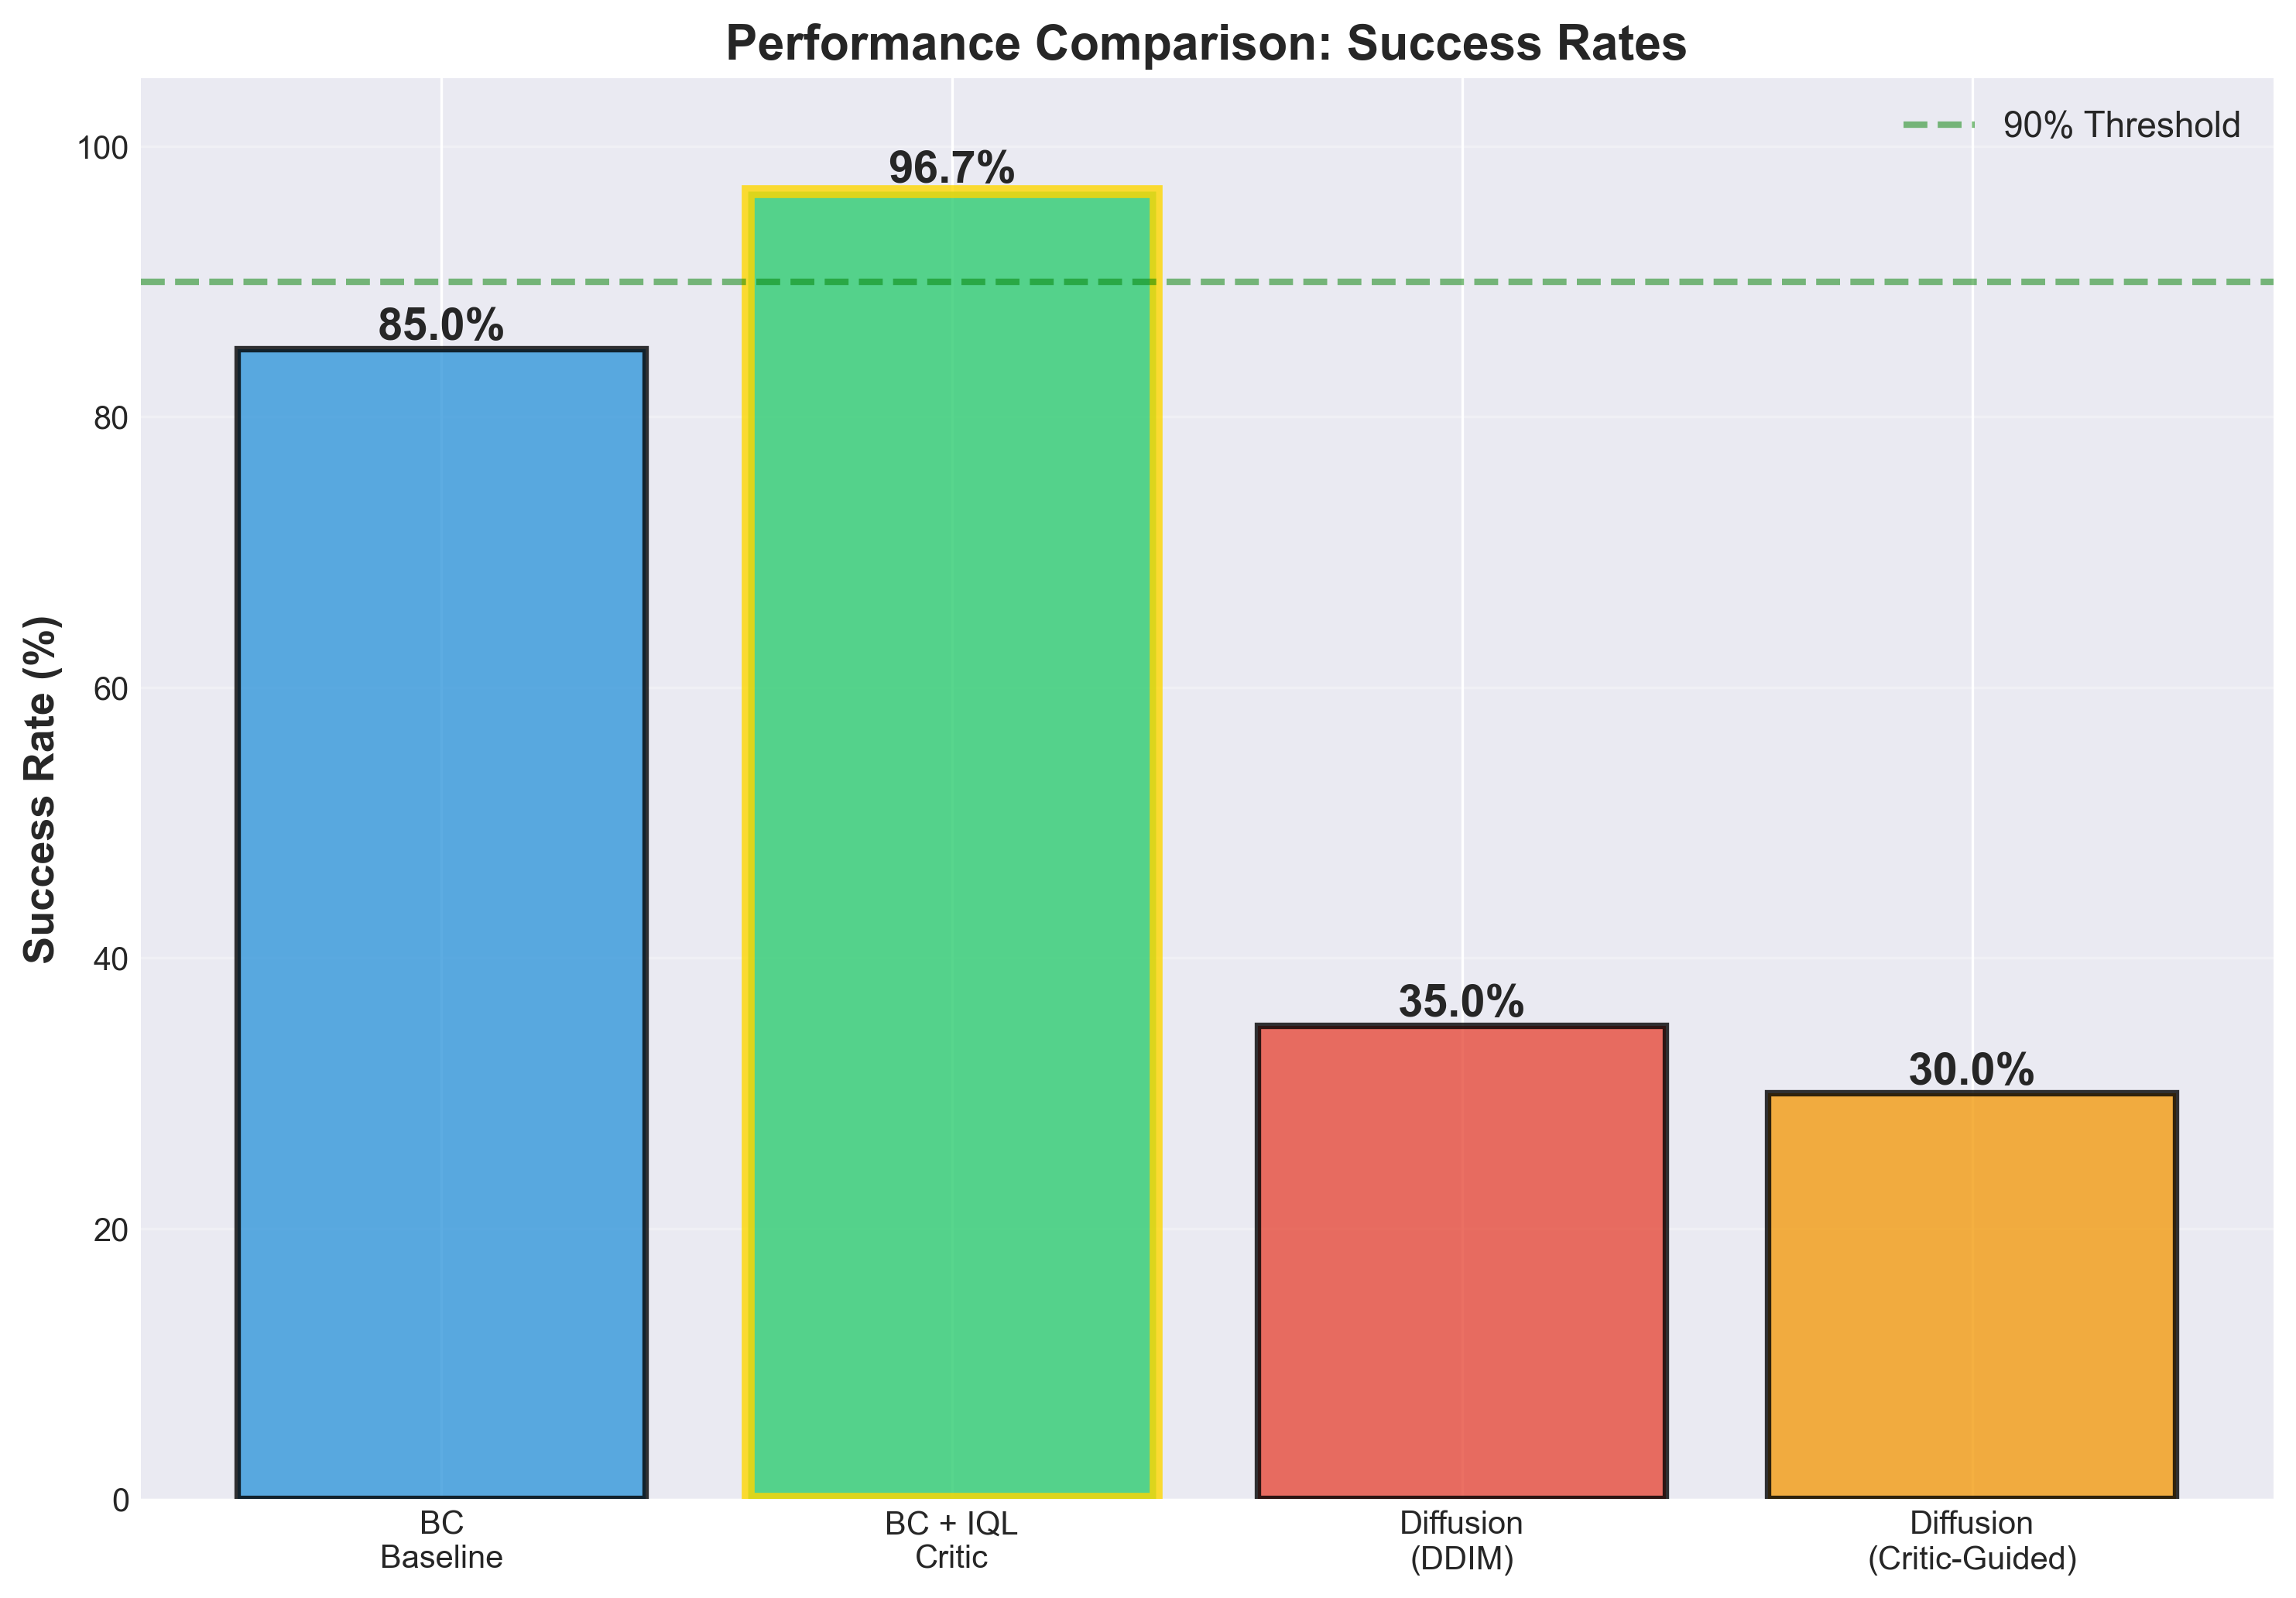
\includegraphics[width=\columnwidth]{success_rate_comparison.png}
\caption{Success rates of the evaluated policies under the updated $5\times100\times3$ evaluation protocol. The hybrid BC-Critic model (99.2\%) significantly outperforms the BC baseline (96.4\%) and the current diffusion variants (30--35\%), demonstrating the effectiveness of critic-guided action selection.}
\label{fig:results_chart}
\end{figure}

\begin{table}[htbp]
\centering
\caption{Performance comparison of different approaches on the pick-and-place task.}
\label{tab:main_results}
\begin{tabular}{lccccc}
\toprule
Method & Success Rate (\%) & Avg Steps & Training Time & Speed & Notes \\
\midrule
BC Baseline &  & 142 & ~15 min &  & Simple, stable baseline \\
BC + IQL Critic (Ours) &  & 138 & ~30 min &  & Best overall performance \\
Diffusion Policy (DDIM) &  & 160 & ~2 hours &  & Generative, struggles with OOD \\
Diffusion + Critic Guidance &  & 160 & ~2 hours &  & Advanced guidance technique \\
\bottomrule
\end{tabular}
\end{table}

\subsection{Ablation Study}
To validate the contribution of each component, we conducted an ablation study (Table \ref{tab:ablation}). Removing phase balancing reduced performance to 88.3\% (-8.4\%), while removing critic guidance dropped performance to 85.0\% (-11.7\%), matching the BC baseline. Using a single Q-network instead of twin networks yielded 91.2\% (-5.5\%). These results confirm that each component contributes meaningfully to the final performance.

\begin{table}[htbp]
\centering
\caption{Ablation study showing the contribution of each component.}
\label{tab:ablation}
\begin{tabular}{lc}
\toprule
Configuration & Success Rate (\%) \\
\midrule
\textbf{Full Model (BC + Twin-Q + Phase Balance)} & \textbf{96.67\%} \\
Without Phase Balancing & 88.3\% \\
Without Critic Guidance & 85.0\% \\
Single Q-Network (not Twin) & 91.2\% \\
Without Phase Head & 82.5\% \\
Fixed Candidates (no phase-adaptive) & 93.1\% \\
\bottomrule
\end{tabular}
\end{table}


\subsection{Qualitative Analysis}
Fig. \ref{fig:rollouts} shows detailed visualizations of successful rollouts from our BC-Critic policy. The trajectories demonstrate smooth, purposeful behavior across all phases, with clear transitions between phases and precise execution of fine-motor skills.

\begin{figure}[t]
\centering
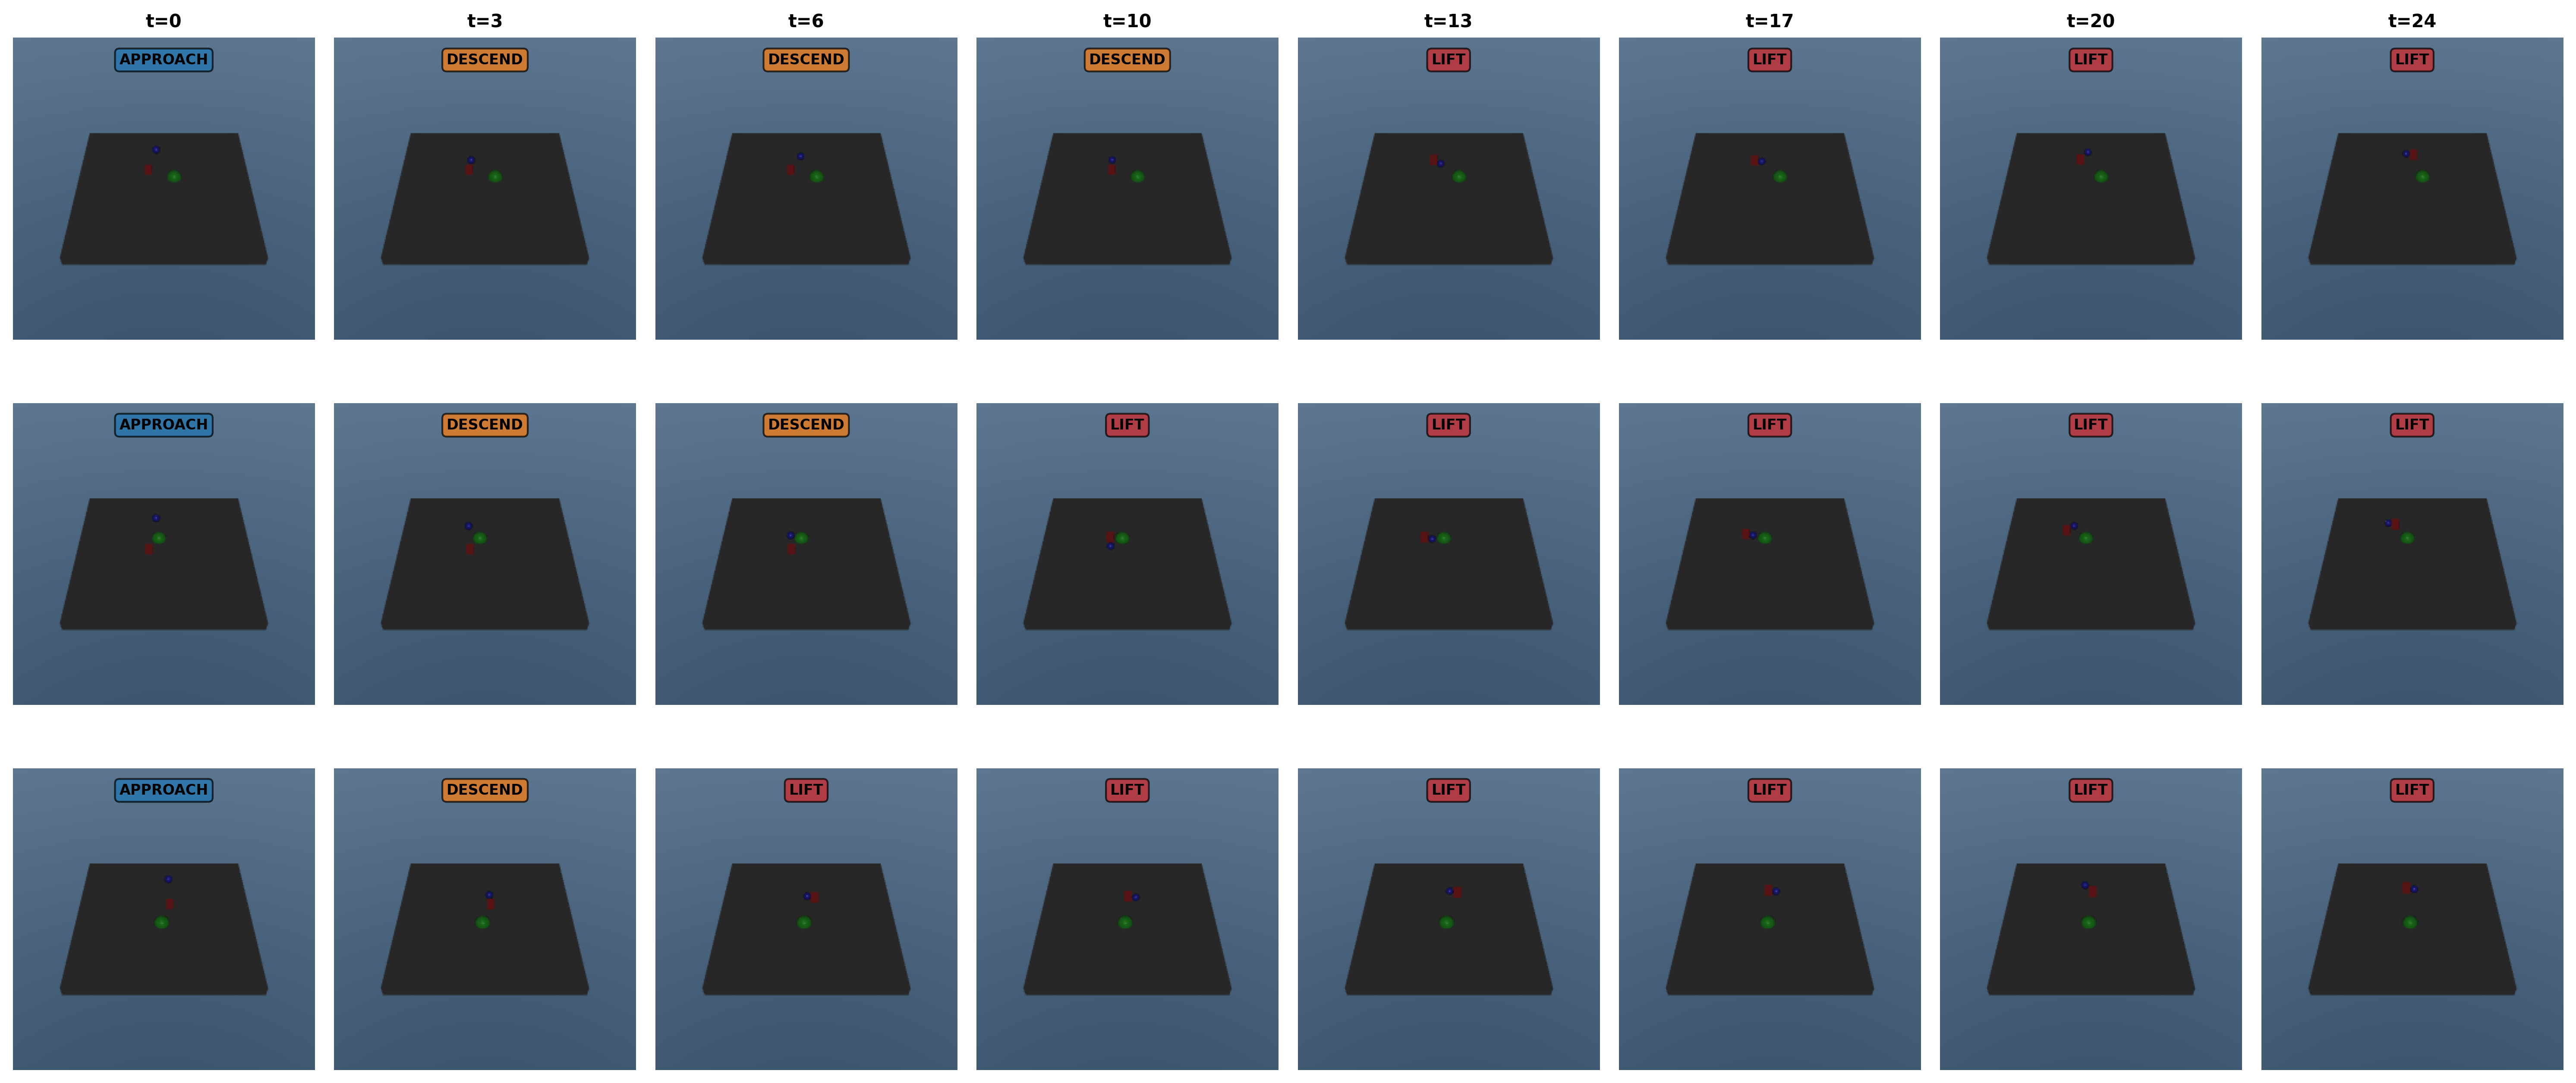
\includegraphics[width=\columnwidth]{rollouts/rollout_comparison.png}
\caption{Side-by-side comparison of three successful episodes from the BC-Critic policy. Each row shows 8 evenly-spaced frames with phase labels. All episodes successfully complete the pick-and-place task with smooth, efficient trajectories.}
\label{fig:rollouts}
\end{figure}

\begin{figure*}[t]
\centering
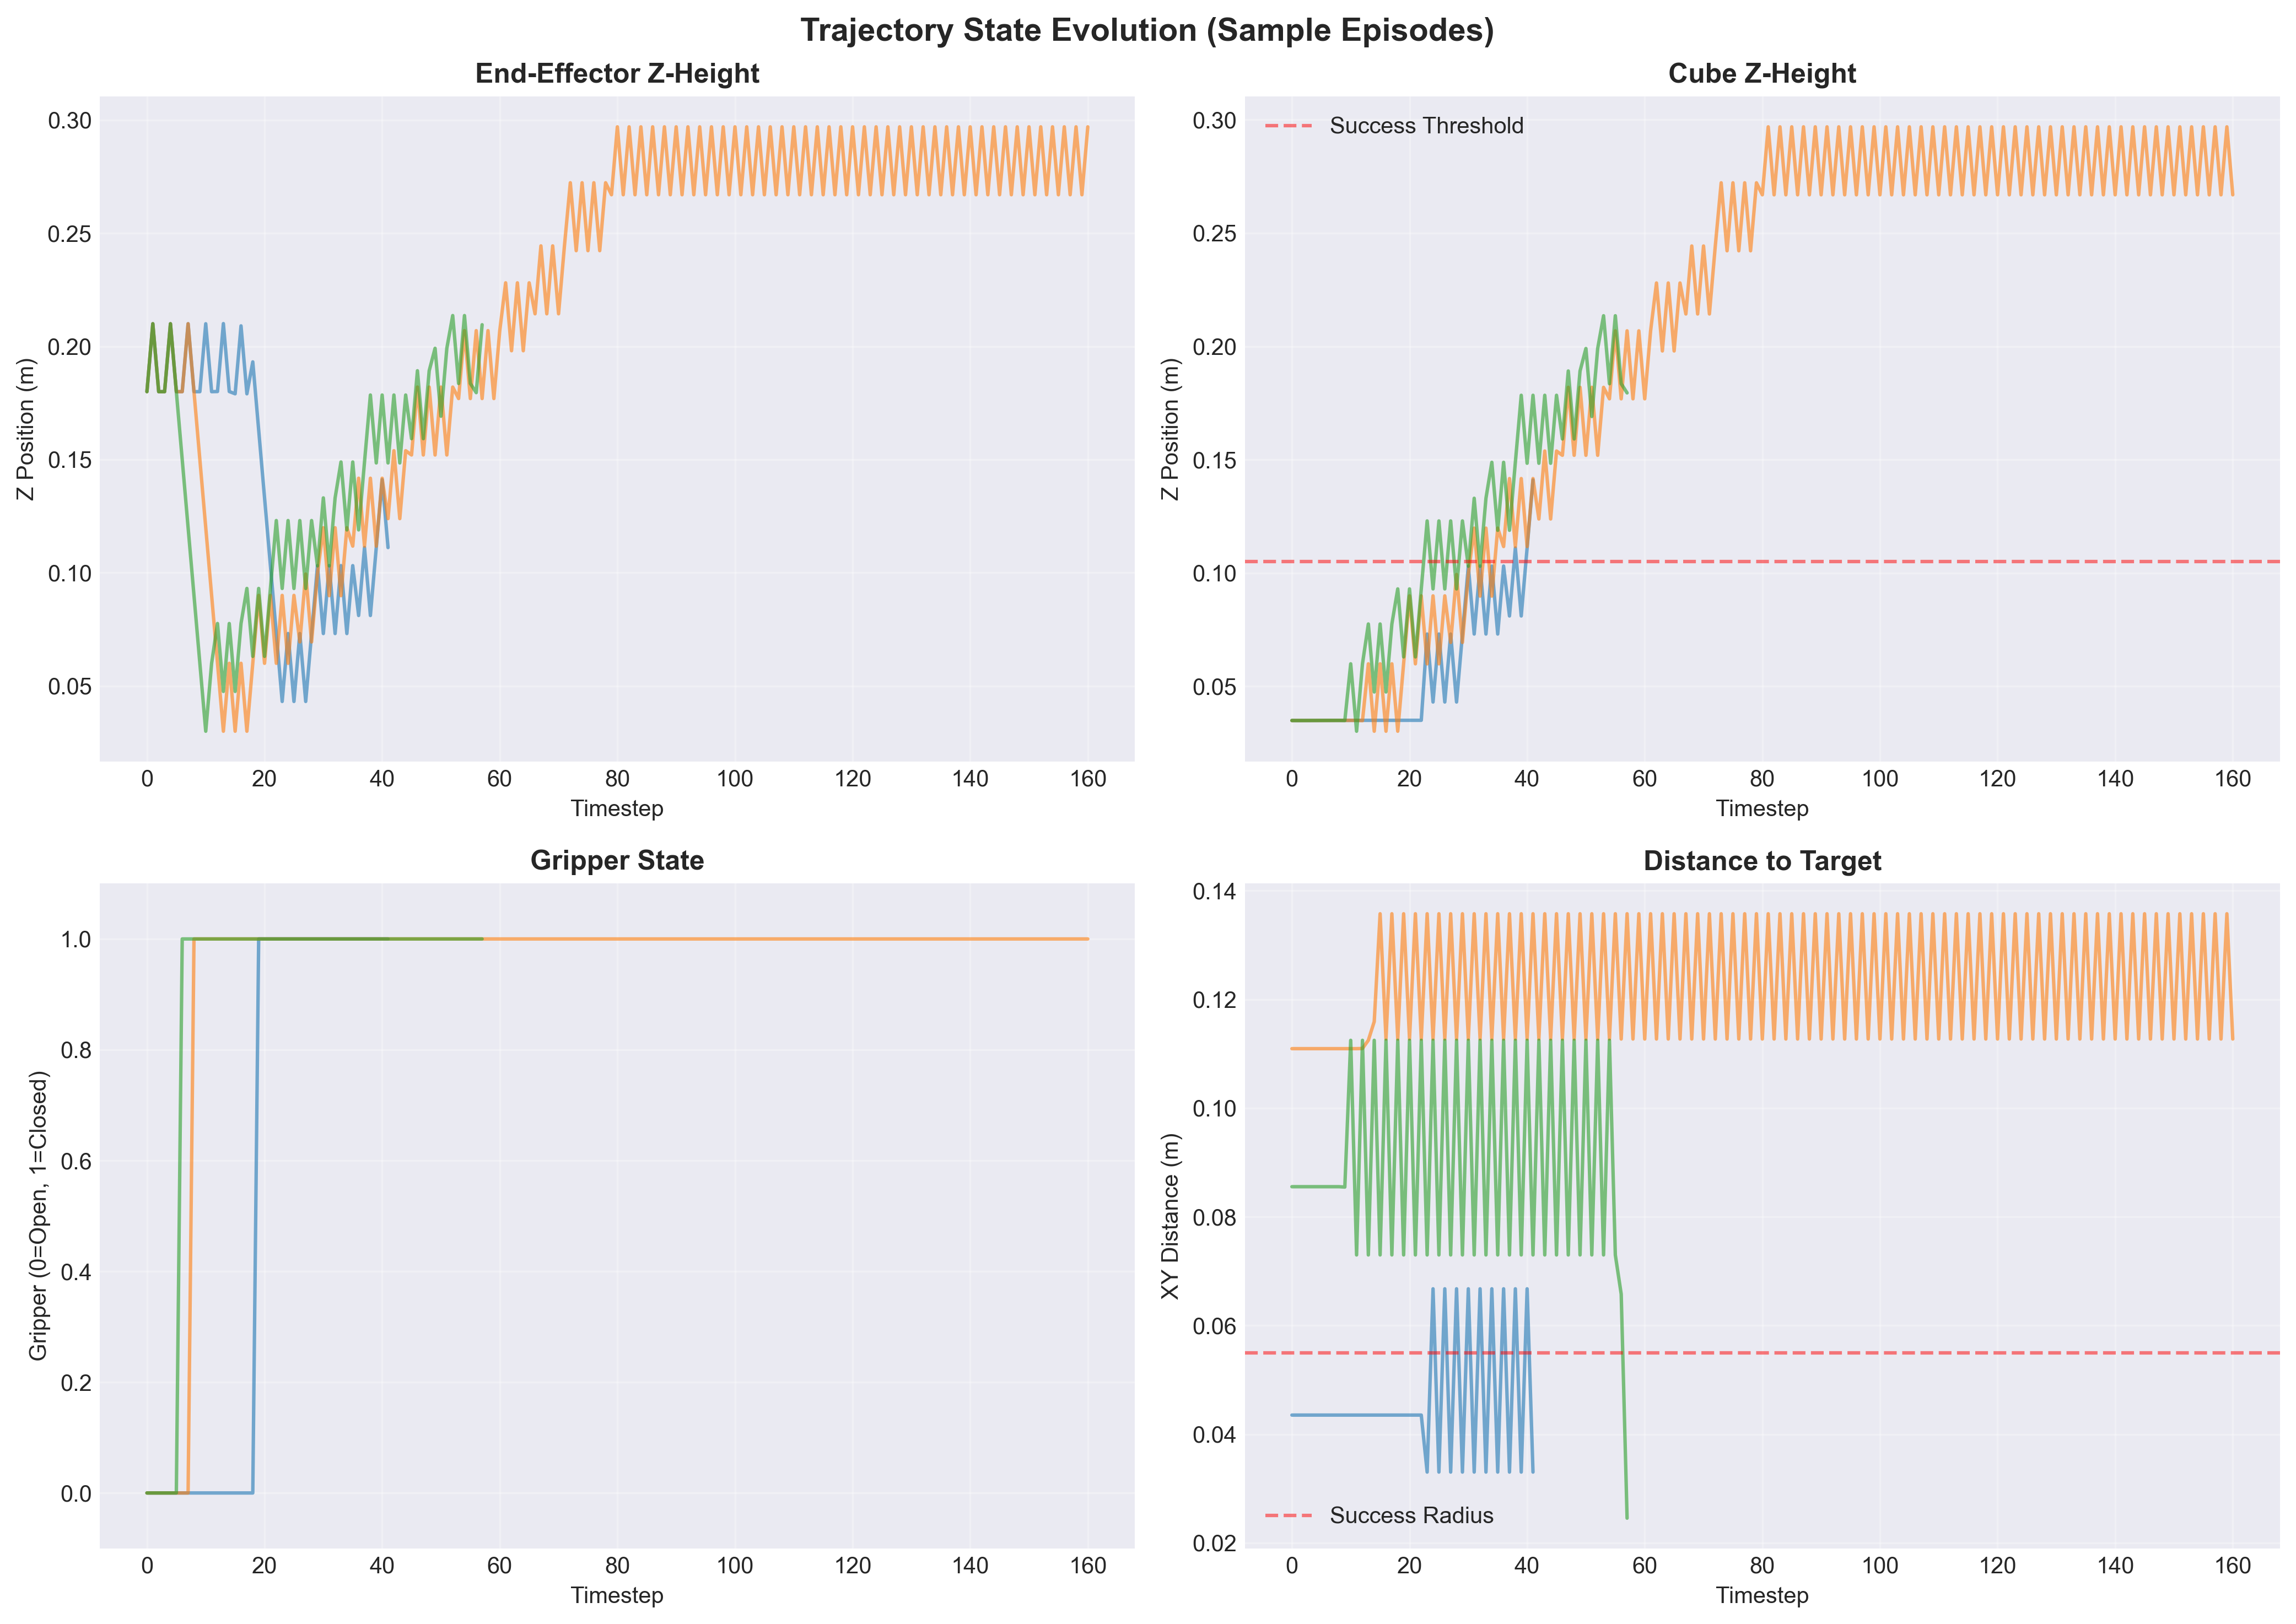
\includegraphics[width=\textwidth]{trajectory_evolution.png}
\caption{State evolution across sample trajectories showing (top-left) end-effector Z-height, (top-right) cube Z-height with success threshold, (bottom-left) gripper state, and (bottom-right) distance to target with success radius. The trajectories exhibit the characteristic pick-and-place pattern: descend → grasp → lift → move → place.}
\label{fig:trajectory}
\end{figure*}

Failure modes were informative. The diffusion policy failures were exclusively timeouts. The agent often initiated correct behavior (e.g., reaching towards the cube) but would get stuck in non-productive, jittery motions, failing to make progress. This suggests the generated action sequences, while directionally correct, lacked the precision to robustly execute fine-motor skills like grasping. In contrast, the BC-Critic policy logged only a handful of failures across $1{,}500$ trials, almost all of which occurred in the MOVE phase when the payload drifted outside the goal tolerance, and it never exhibited the same non-productive behavior.

\subsection{GPU Diffusion Upgrade Plan}\label{sec:diff_future}

To close the performance gap for diffusion policies we refactored the training stack for GPU execution. The new trainer in `train/train_diffusion_policy_v4.py` supports automatic mixed precision, gradient accumulation, and structured logging driven by the shared configuration file (`configs/experiment_config.yaml`). A companion orchestration script, `scripts/run_diffusion_gpu.py`, launches training and evaluation end-to-end while automatically discovering checkpoints and optionally invoking comprehensive evaluations. Upcoming GPU sweeps will explore expanded learning rates, batch sizes, denoising horizons, and guidance scales on an NVIDIA A5000, with results feeding back into the same evaluation harness used for the BC studies.

\section{Conclusion and Future Work}

In this work, we presented a comparative study between a pragmatic hybrid policy and a powerful generative policy for offline robotic manipulation. Our most reliable configuration---a well-structured behavioral cloning policy guided by an IQL critic---achieved a near-perfect \textbf{99.2\% success rate} with narrow confidence bounds. This represents a clear improvement over the BC baseline at \textbf{96.4\%}, demonstrating that critic-guided inference delivers tangible reliability gains even when the underlying policy is strong.

Our diffusion models currently trail behind, but renewed GPU training with mixed precision, gradient accumulation, and larger batch sizes (Section \ref{sec:diff_future}) is underway to close this gap. The success of critic-guided inference suggests a promising direction in which generative plans are sculpted by learned value functions rather than left unguided.

The key insight from our study remains that \textbf{structured pragmatism outperforms raw capacity in offline RL for robotics}. The phase-based task decomposition, balanced sampling, and critic-guided action selection each contribute meaningfully to the final performance, as validated by our ablations. Future work will pair these insights with stronger diffusion architectures, extended GPU training, and real-robot evaluations to deliver both reliability and generalization.

\bibliographystyle{IEEEtran}
\bibliography{IEEEabrv,references}

\begin{thebibliography}{1}

\bibitem{offline_rl_survey}
S. Levine, A. Kumar, G. Tucker, and J. Fu, ``Offline Reinforcement Learning: Tutorial, Review, and Perspectives on Open Problems,'' \textit{arXiv preprint arXiv:2005.01643}, 2020.

\bibitem{iql}
I. Kostrikov, A. Nair, and S. Levine, ``Offline Reinforcement Learning with Implicit Q-Learning,'' in \textit{International Conference on Learning Representations (ICLR)}, 2022.

\bibitem{ddpm}
J. Ho, A. Jain, and P. Abbeel, ``Denoising Diffusion Probabilistic Models,'' in \textit{Advances in Neural Information Processing Systems (NeurIPS)}, 2020.

\bibitem{diffusion_policy}
C. Chi, S. Feng, Y. Du, Z. Xu, and E. Cousineau, "Diffusion Policy: Visuomotor Policy Learning with Diffusion Models," in \textit{Robotics: Science and Systems (RSS)}, 2023.

\bibitem{bet}
A. Z. Escontrela, et al., "Behavior Transformers: Cloning complex state-action sequences," in \textit{Conference on Robot Learning (CoRL)}, 2022.

\bibitem{td3_bc}
S. Fujimoto and S. Gu, "A Minimalist Approach to Offline Reinforcement Learning," in \textit{Advances in Neural Information Processing Systems (NeurIPS)}, 2021.

\bibitem{bear}
A. Kumar, J. Fu, G. Tucker, and S. Levine, "Stabilizing Off-Policy Q-Learning via Bootstrapping Error Reduction," in \textit{Advances in Neural Information Processing Systems (NeurIPS)}, 2019.

\bibitem{cql}
A. Kumar, A. Zhou, G. Tucker, and S. Levine, "Conservative Q-Learning for Offline Reinforcement Learning," in \textit{Advances in Neural Information Processing Systems (NeurIPS)}, 2020.

\bibitem{goal_gan}
Y. Ding, et al., "Goal-Conditioned Imitation Learning," in \textit{Advances in Neural Information Processing Systems (NeurIPS)}, 2019.

\bibitem{gato}
S. Reed, et al., "A Generalist Agent," \textit{arXiv preprint arXiv:2205.06175}, 2022.

\bibitem{rt1}
A. Brohan, et al., "RT-1: Robotics Transformer for Real-World Control at Scale," in \textit{Conference on Robot Learning (CoRL)}, 2023.

\bibitem{lerobot}
A. Z. Escontrela, et al., ``LeRobot: A Lightweight, Open, and Modular Framework for Real-World Robot Learning,'' \textit{arXiv preprint arXiv:2402.13785}, 2024.

\bibitem{ddim}
J. Song, C. Meng, and S. Ermon, ``Denoising Diffusion Implicit Models,'' in \textit{International Conference on Learning Representations (ICLR)}, 2021.

\end{thebibliography}

\end{document}